\documentclass[compress]{beamer}
%--------------------------------------------------------------------------
% Common packages
%--------------------------------------------------------------------------
\usepackage[german]{babel}
\usepackage[T1]{fontenc}
\usepackage{graphicx}
\usepackage{multicol}
\usepackage{amsmath}
\usepackage{color}



% Erweiterte Tabellenfunktionen
\usepackage{tabularx,ragged2e}
\usepackage{booktabs}
% for the transition diagram
\usepackage{tikz}
\usetikzlibrary{arrows}
\setbeameroption{show notes}
% Listingserweiterung
\usepackage{listings}
\lstset{ %
  language=[LaTeX]TeX,
  basicstyle=\normalsize\ttfamily,
  keywordstyle=,
  numbers=left,
  numberstyle=\tiny\ttfamily,
  stepnumber=1,
  showspaces=false,
  showstringspaces=false,
  showtabs=false,
  breaklines=true,
  frame=tb,
  framerule=0.5pt,
  tabsize=4,
  framexleftmargin=0.5em,
  framexrightmargin=0.5em,
  xleftmargin=0.5em,
  xrightmargin=0.5em
}


% ------------------------------------------------------------------------------
%  Tikz
% ------------------------------------------------------------------------------
\usetikzlibrary{arrows,positioning}
\tikzset{
  %Define standard arrow tip
  >=stealth',
  %Define style for boxes
  punkt/.style={
    rectangle,
    rounded corners,
    draw=black, very thick,
    text width=6.5em,
    minimum height=2em,
    text centered},
  % Define arrow style
  pil/.style={
    ->,
    thick,
    shorten <=2pt,
    shorten >=2pt,}
}

%   NaturProzess




\newcommand{\captionslide}[1]{
  {\setbeamercolor{background canvas}{bg=hsrmWarmGreyLight}
    \begin{frame}[plain]
      \addtocounter{framenumber}{-1}
      \begin{center}
        \vfill\usebeamerfont{section title}\textcolor{black}{\MakeUppercase{#1}}\vfill
      \end{center}
    \end{frame}
  }
}



%--------------------------------------------------------------------------
% Load theme
%--------------------------------------------------------------------------
\usetheme[nosectionpages]{hsrm}


\usepackage{dtklogos} % must be loaded after theme
\usepackage{tikz}

%\title{Überblick Maschinelles Lernen}
\title{Statistische Modellierung: Die zwei Kulturen}
\subtitle{Seminar für Statistische Modellierung latenter Strukturen in den Lebens-, Sozial- und Wirtschaftswissenschaften}
\date{18.01.2013, 12:30 Uhr \\Seminarraum, Institut für Statistik, LMU}
\author{Christoph Molnar \\ Betreuer: Georg Schollmeyer \\ Seminarleiter: Professor Augustin}

\begin{document}


\maketitle
\addtocounter{framenumber}{-1}
\note{
\textbf{Abstract:} \\
In der Präsentation werden zwei Kulturen der Modellierung verglichen: die Datenmodellierung, bei der ein datengenerierender stochastischer Prozess angenommen wird und die mit traditioneller Statistik assoziiert ist; die algorithmische Modellierung, die auf Optimierung einer Funktion mit Hilfe eines Algorithmus reduziert werden kann und mit Machine Learning assoziiert wird. \\ Es wird für stärkere Verwendung von algorithmischer Modellierung in der Statistik argumentiert. 
}

\begin{frame}{Gliederung}
  \begin{enumerate}
  \item Statistik: Kultur der Datenmodellierung
  \item Machine Learning: Kultur der algorithmischen Modellierung
  \item Prinzipien beim Lernen aus Daten
  \item Persönliche Erfahrungen
  \item Fazit
  \end{enumerate}
  \let\thefootnote\relax\footnotetext{Inhalt basiert auf: ``Statistical Modeling: The two cultures'' von  Leo~Breiman \cite{breiman}}
\end{frame}

\note{
Die Präsentation basiert auf dem Artikel ``Statistical Modeling: The two cultures'' von Leo Breiman \cite{breiman}. \\ Im ersten Abschnitt wird die Modellierung in der Statistik betrachtet und analog dazu im zweiten Abschnitt die Modellierung im Machine Learning inklusive kurzer Vorstellung einiger Algorithmen. Das Kapitel über Prinzipien beim Lernen aus Daten stellt die beiden Kulturen gegenüber. Persönliche Erfahrungen illustrieren Beispiele für die beiden Kulturen. Im Fazit wird die Botschaft des Artikels \cite{breiman} zusammengefasst. 
}


\section{Statistik}
\captionslide{Statistik: Kultur der Datenmodellierung}



\begin{frame}[fragile]\frametitle{Arbeit eines Statistikers}
  \begin{itemize}
  \item \textbf{Prognosen treffen}
  \item \textbf{Zusammenhänge erklären}
  \item Versuchsplanung, Parameterschätzung, Visualisierung, \ldots
  \end{itemize}
\end{frame}

\note{
Die Arbeit eines Statistikers ist sehr vielfältig. Hier wird nur über die Modellierung der Daten gesprochen, die zwei Ziele hat: 
Prognose für neue Beobachtungen und Erklärung von Zusammenhängen. 
}


\begin{frame}[fragile]\frametitle{Vereinfachtes Weltbild}
  \begin{center}
    \begin{tikzpicture}[->,>=stealth',shorten >=1pt,auto,node distance=1cm,
        thick,main node/.style={circle,fill=blue!20,draw,font=\sffamily\Large\bfseries}]
      \node[punkt] (natur) {Natur};
      \node[right=of natur] (x) {Kovariablen};
      \node[left=of natur] (y) {Zielgröße};
      \path[every node/.style={font=\sffamily\small}]
      (natur) edge node {} (y)
      (x) edge node  {} (natur)
      ;
    \end{tikzpicture} \\
  \end{center}
\end{frame}

\note{
 Vereinfacht kann die Natur als ein Mechanismus in einer Box betrachtet werden, der aus Kovariablen die Zielgröße generiert. 
 Die Kenntnisse über den Mechanismus der Natur können von vollkommen unbekannt bis hin zu etablierten substanzwissenschaftlichen Theorien reichen. Ein Beispiel ist der Mietspiegel: Hier ist die Zielgröße der Mietpreis und Kovariablen sind Größe und Alter der Wohnung, Art der Heizung, \ldots
}


\begin{frame}[fragile]\frametitle{Weltbild des Statistikers}
  \begin{center}
    \begin{tikzpicture}[->,>=stealth',shorten >=1pt,auto,node distance=1cm,
        thick,main node/.style={circle,fill=blue!20,draw,font=\sffamily\Large\bfseries}]
      \node[punkt] (natur) {Logistische Regression, \\Cox Model, \\GEE, \\ \ldots};
      \node[right=of natur] (x) {Kovariablen};
      \node[left=of natur] (y) {Zielgröße};
      \path[every node/.style={font=\sffamily\small}]
      (natur) edge node {} (y)
      (x) edge node  {} (natur)
      ;
    \end{tikzpicture}
  \end{center}
  Suche stochastisches Modell der Daten: \\
  Zielgröße = f(Kovariablen, Parameter, zufälliger Fehler)
\end{frame}

\note{
  Das direkte Modellieren des Mechanismus in der ``Box'' wird von Breiman als \doublequoted{Data Modeling Culture} bezeichnet. In dieser Kultur wird für den datengenerierenden Prozess ein stochastisches Modell angenommen, dessen Parameter geschätzt werden können. Die meisten Modelle sind so formuliert, dass die Zielgröße eine Funktion der Kovariablen mit dazugehörigen Parametern und einem Fehlerterm ist. 
}


\begin{frame}[fragile]\frametitle{Typische Annahmen und Restriktionen}
  \begin{itemize}
  \item Stochastisches Modell, dass Daten generiert
  \item Bestimmte Verteilung der Residuen
  \item Linearitäten (z.B. Linearer Prädiktor)
  \item Interaktionen müssen manuell spezifiert werden 
  \end{itemize}
\end{frame}


\begin{frame}[fragile]\frametitle{Probleme}
  \begin{itemize}
  \item Schlussfolgerungen über Modellmechanismen, nicht über Natur
  \item Annahmen häufig verletzt
  \item Häufig keine Modellevaluierung
  \item $\Rightarrow$ führt zu irrelevanter Theorie und fragwürdigen statistischen Schlussfolgerungen
  \item Fokus nicht auf Prognosekraft
  \item Datenmodelle ungenügend in Gebieten wie Bilderkennung, Spracherkennung, \ldots
  \end{itemize}
\end{frame}

\section{Machine Learning}
\captionslide{Machine Learning: Kultur der algorithmischen Modellierung}

\begin{frame}{Machine Learning}
  \begin{center}
    \begin{tikzpicture}[->,>=stealth',shorten >=1pt,auto,node distance=1cm,
        thick,main node/.style={circle,fill=blue!20,draw,font=\sffamily\Large\bfseries}]
      \node[punkt] (natur) {unbekannt};
      \node[right=of natur] (x) {Kovariablen X};
      \node[left=of natur] (y) {Zielgröße Y};
      \node[below=of natur, label=below:Algorithmus] (algo) { \includegraphics*[width = 3cm]{./images/machine.png}};
      \path[every node/.style={font=\sffamily\small}]
      (natur) edge node {} (y)
      (x) edge node  {} (natur)
      (x) edge[<->, bend left=30] node {} (algo)
      (y) edge[<->, bend right=30] node {} (algo)
      ;
    \end{tikzpicture}
  \end{center}
  Suche Funktion $f(X)$ die den Verlust $L(Y, f(X))$ minimiert
\end{frame}

\note{
  Bei dem von Breiman als \doublequoted{Algorithmic Modeling Culture} bezeichneten Vorgehen sieht man den tatsächlichen Mechanismus als unbekannt an. Man versucht nicht den datengenerierenden Prozess zu finden, sondern benutzt einen Algorithmus um den Mechanismus der Natur zu imitieren. Die Modellierung reduziert sich zu einem mathematischen Optimierungsproblem: Gegeben Kovariablen, Zielgröße und Verlustfunktion, suche ein Funktion f(X), die den Verlust bei der Vorhersage der Zielgröße minimiert. Diese Kultur findet man im Bereich des Machine Learning. \\
Zusammenfassung: Datenmodellierung versucht den wahren Mechanismus zu finden, algorithmische Modellierung versucht den wahren Mechanismus möglichst gut zu imitieren. 
}

\begin{frame}[fragile]\frametitle{Algorithmen im Machine Learning}
  \begin{itemize}
  \item Boosting
  \item Support Vector Machines
  \item Künstliche Neuronale Netze
  \item Random Forests
  \item Hidden Markov
  \item Bayes-Netze
  \item \ldots{} \footnote{Details und mehr Algorithmen in ``Elements of statistical learning''\cite{elements}}
  \end{itemize}

\end{frame}

\note{
Die Algorithmen im Machine Learning unterscheiden sich von den Ideen her sehr stark. Drei Algorithmen werden im Folgenden kurz vorgestellt. 
}


\begin{frame}{Künstliche neuronale Netze}
  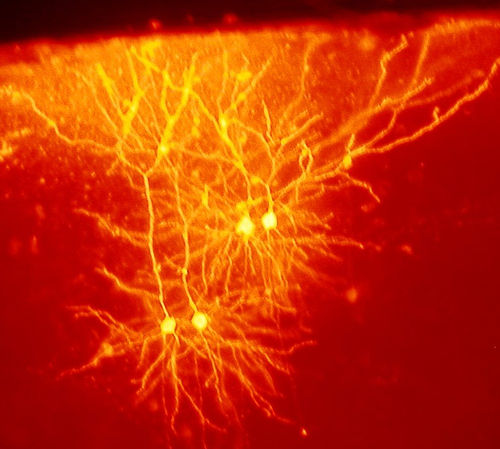
\includegraphics[width = 5cm]{./images/neurons.jpg}
  \hspace*{0.6cm}
  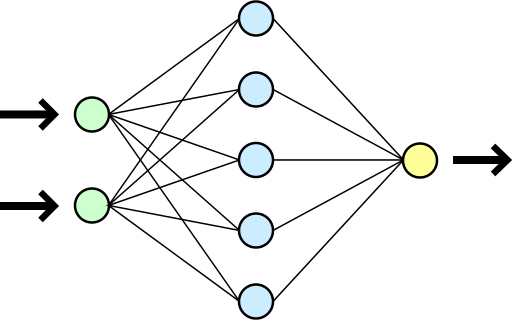
\includegraphics[width = 5cm]{./images/ANN.png}
  \footnote{\url{http://commons.wikimedia.org/wiki/File:Mouse_cingulate_cortex_neurons.jpg} \\ \url{http://commons.wikimedia.org/wiki/File:Neural_network.svg}}
\end{frame}

\note{
Künstliche neuronale Netze können für Klassifikation und Regression benutzt werden. Sie sind inspiriert durch das Gehirn, das aus Netzwerken von Gehirnzellen (Neuronen) besteht. Mathematisch sind künstliche neuronale Netze Verkettungen von gewichteten Funktionen. 
Typisches Anwendungsgebiet ist die Bildverarbeitung.}

\begin{frame}{Support Vector Machines}
  \begin{center}
    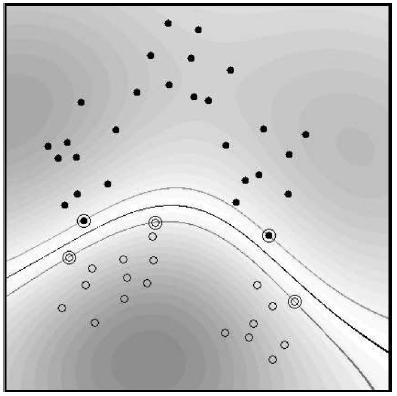
\includegraphics[width = 7cm]{./images/SVM.JPG}
    \footnote{\url{http://commons.wikimedia.org/wiki/File:Svm_10_perceptron.JPG}}
  \end{center}
\end{frame}

\note{
Eine Support Vector Machine (SVM) ist ursprünglich ein Klassifikationsverfahren (Regression auch möglich). Sie funktioniert so, dass sie versucht im Raum der Kovariablen eine Klassengrenze zu ziehen, wobei der Abstand der Grenze zu den Beobachtungen maximiert wird. SVMs benutzen einen mathematischen Trick um implizit die Kovariablen in einen höherdimensionalen Raum abzubilden und so Trennbarkeit der Klassen zu erreichen. Typisches Anwendungsgebiet: Klassifikation von Text
}

\begin{frame}{Random Forests}
  \begin{center}
    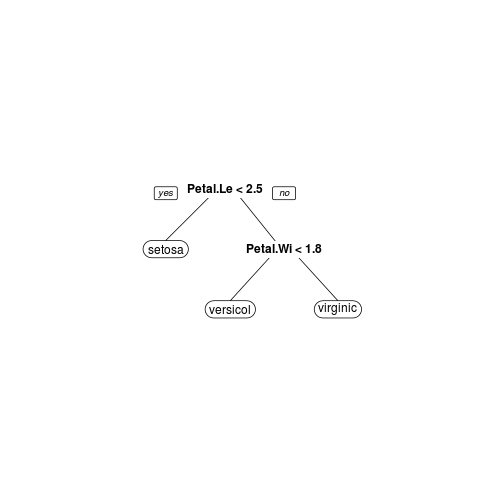
\includegraphics[width = 10cm, clip, trim = 3cm 0cm 3cm 4cm]{./images/tree.png}
  \end{center}
\end{frame}

\begin{frame}{Random Forests}
  \begin{center}
    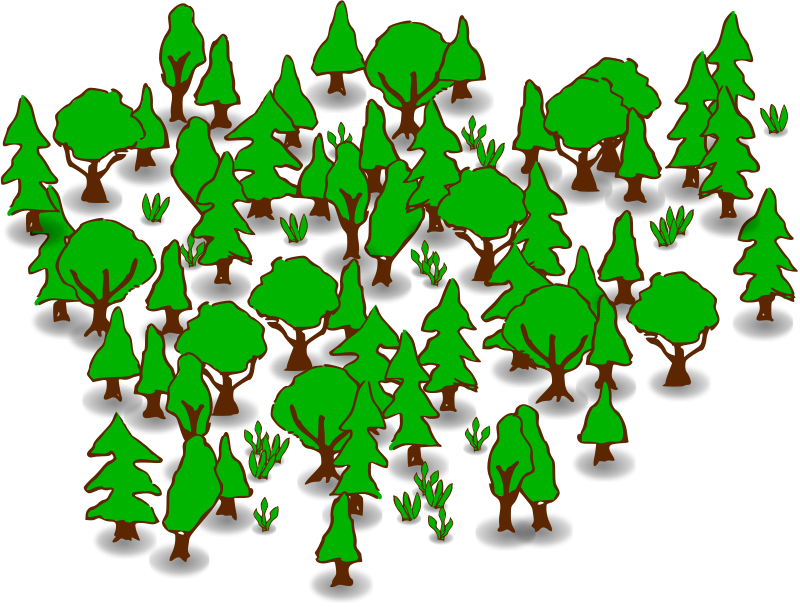
\includegraphics[width = 10cm]{./images/forest.png}
    \footnote{\url{http://openclipart.org/detail/175304/forest-by-z-175304}}
  \end{center}
\end{frame}

\note{
  Random Forests\texttrademark (Erfinder: Leo Breiman) werden für Regressions- und Klassifikationsprobleme eingesetzt. Ein Random Forest setzt sich aus vielen Entscheidungsbäumen zusammen. Es gibt zwei Zufallsmechanismen, die dazu benutzt werden um unterschiedliche Entscheidungsbäume an die Daten anzupassen. Für die Vorhersage werden die Vorhersagen aller Bäume aggregiert. 
}

\section{Prinzipien}
\captionslide{Prinzipien beim Lernen aus Daten}

%% \begin{frame}[fragile]\frametitle{Prinzipien}
%%   \begin{itemize}
%%   \item Statistik: Bemühung der Reduktion von Kovariablen (Selektion, Dimensionsreduktion)
%%   \item Machine Learning: Je mehr Variable, desto besser
%%   \item Rashomon: Die Vielfalt guter Modelle
%%   \item Occam ???
%%   \end{itemize}
%% \end{frame}

\begin{frame}{Rashomon Effekt}
  \begin{center}
    Es gibt meist viele unterschiedliche Modelle, die einen Sachverhalt gleich gut beschreiben.
  \end{center}
\end{frame}

\note{
  Rashomon ist ein japanischer Film, in dem 4 Zeugen unterschiedliche Versionen von einem beobachteten Verbrechen erzählen. Alle Versionen erklären die Fakten und doch sind alle widersprüchlich. \\ Übertragen auf das statistische Lernen bedeutet das, dass unterschiedliche Modelle (z.B. mit unterschiedlichen Kovariablen) die Daten gleich gut vorhersagen. Jedes Modell hat aber eine andere Interpretation. \\
  Algorithmen wie Random Forest und Boosting nutzen diesen Effekt aus und aggregieren über viele Modelle. Außerdem ist es im Machine Learning gängige Praxis verschiedene Algorithmen zu benutzen und die Resultate für die Vorhersage zu aggregieren.
}

\begin{frame}{Dimensionalität der Daten}
  \begin{itemize}
  \item Je höher die Dimensionalität (\# Kovariablen) desto schwieriger das Trennen von Rauschen und Einflüssen
  \item Gängige Praxis in der Statistik: Variablenselektion (theoretisch motiviert oder datengesteuert) und Dimensionsreduktion
  \item Gängige Praxis im Machine Learning: Erzeugen von vielen neuen Kovariablen um Vorhersage zu verbessern; Algorithmen meist robust für hochdimensionale Daten
  \end{itemize}
\end{frame}

\note{
  Random Forest robust durch Aggregation von vielen Modellen und Randomisierung bei Variablenwahl.
  Support Vector Machines erzeugen sogar absichtlich höhere Dimensionalitäten der Daten um Trennbarkeit zu erreichen
}


\begin{frame}{Vorhersage vs. Interpretierbarkeit}
  \begin{tikzpicture}
    \draw (0,0) -- (0,1.5) -- (9.9,0) -- (0,0);
    \draw  (0, 1.6) -- (10,1.6) -- (10, 0.1) -- (0, 1.6);
    \node at (3, 0.2) {Interpretierbarkeit};
    \node at (7, 1.3) {Vorhersagegüte};
    \node at (1.3, -0.5) {Tree};
    \node at (9, -0.5) {Random Forest};
    \node at (1.5, -1.2) {Logist. Regression};
    \node at (9, -1.2) {Neuronales Netz};
    \node at (1.3, -1.9) {\ldots};
    \node at (9, -1.9) {\ldots};
  \end{tikzpicture}
\end{frame}

\note{
  Es gibt einen Tradeoff zwischen Interpretierbarkeit und Vorhersagekraft von Modellen: Komplexere Modelle liefern häufig genauere Vorhersagen. Gut interpretierbare Methoden sind meist schlecht in der Vorhersage.
  Ein Beispiel sind Entscheidungsbäume und Random Forests: Ein einzelner Entscheidungsbaum ist sehr intuitiv und auch für Laien leicht zu interpretieren, dafür sind sie sehr instabil und liefern nicht so gute Vorhersagen. Ein Aggregat von zufällig erzeugten Bäumen, ein Random Forest, hat eine ausgezeichnete Vorhersagegüte, aber die Modellstruktur lässt sich nicht mehr interpretieren. 
}

\begin{frame}{Modellgüte}
  \begin{itemize}
  \item Statistik: Gütekriterien beruhen häufig auf Modellannahmen und werden auf Trainingsdaten berechnet. Manchmal gar keine Evaluierung
  \item Machine Learning: Gängige Praxis: Kreuzvalidierung, extra Testset
  \end{itemize}
  Wie gut ist ein statistisches Modell wenn die Vorhersagegüte schlecht ist? Darf man Parameter und p-Werte interpretieren?
\end{frame}

%% \note{
%%   Direkteste Messung wie gut das Modell die ``Natur abbildet'':
%%   Nimm Beobachtung x und beobachte von der Natur produziertes y, mach das gleiche mit dem Model und beobachte y'. 
%%   Vergleiche y' mit y. \\
%%   In Statistik werden häufig likelihood-basierte Kriterien verwendet. 
%% }


\section{Erfahrungen}
\captionslide{Persönliche Erfahrungen}

\begin{frame}[fragile]\frametitle{Statistische Beratung}
  Stereotypische Anwender ...
  \begin{itemize}
  \item sind z.B. Tiermediziner, Linguisten, Biologen, \ldots
  \item sehnen sich nach p-Werten für Koeffizienten
  \item möchten Interpretierbarkeit, keine Vorhersagegüte
  \item haben meist Erfahrung mit linearen Modellen (kein Machine Learning)
  \item kümmeren sich nicht um Modelldiagnose
  \end{itemize}
\end{frame}

\note{
  Vor allem in der Forschung möchten Anwender Hypothesen mit Hilfe von Modellen überprüfen. Dabei ist meistens nicht von Interesse wie gute Vorhersagen ein Modell liefert, sondern z.B. auf welche Werte die Koeffizienten geschätzt wurden und ob sie signifikant sind. Algorithmische Modellierung ist hier in den meisten Fällen wegen mangelnder Interpretierbarkeit nicht interessant. 
}

\begin{frame}[fragile]\frametitle{kaggle}
  Algorithmen der Gewinner auf kaggle, Plattform für Prognose-Wettbewerbe:
  \begin{itemize}
    % http://blog.kaggle.com/2013/05/06/qa-with-job-salary-prediction-first-prize-winner-vlad-mnih/
  \item  Job Salary Prediction: \doublequoted{I used deep neural networks}
    % http://blog.kaggle.com/2012/12/19/1st-place-observing-dark-worlds/
  \item Observing Dark Worlds: \doublequoted{Bayesian analysis provided the winning recipe for solving this problem}
    % http://blog.kaggle.com/2012/01/03/the-perfect-storm-meet-the-winners-of-give-me-some-credit/
  \item Give Me Some Credit: \doublequoted{In the end we only used five supervised learning methods: a random forest of classification trees, a random forest of regression trees, a classification tree boosting algorithm, a regression tree boosting algorithm, and a neural network.}
  \end{itemize}
\end{frame}

\note{
Kaggle (\url{http://www.kaggle.com}) ist eine Internetplattform auf der Vorhersageprobleme als Wettbewerbe ausgeschrieben werden. Daten werden zur Verfügung gestellt und es gewinnt derjenige, dessen Vorhersage auf Testdaten am Besten war. Es ist nicht teil des Wettbewerbes relevante Einflussgrößen zu identifizieren oder Erkenntnisse über den datengenerierenden Prozess zu finden. Da hier nur die Vorhersage zählt ist die algorithmische Modellierung klar im Vorteil gegenüber der Kultur der Datenmodellierung. 
}

\section{Fazit}
\begin{frame}{Fazit}
  Ein Statistiker sollte:
  \begin{itemize}
  \item Modelle kritisch evaluieren
  \item Prognosegüte als Kriterium für die Modellgüte benutzen
  \item Das beste Modell suchen, egal ob aus der Statistik oder Machine Learning
  \item Machine Learning in die Toolbox mit aufnehmen.
  \item Sich immer bewusst machen: \\ \doublequoted{All models are wrong, but some are useful} (G. Box)
  \end{itemize}
\end{frame}


\begin{frame}{Weiterführende Literatur}
  %% @article{breiman2001statistical,
  %%   title={Statistical modeling: The two cultures (with comments and a rejoinder by the author)},
  %%   author={Breiman, Leo},
  %%   journal={Statistical Science},
  %%   volume={16},
  %%   number={3},
  %%   pages={199--231},
  %%   year={2001},
  %%   publisher={Institute of Mathematical Statistics}
  %% }

  %% @book{trevor2001elements,
  %%   title={The elements of statistical learning},
  %%   author={Trevor. Hastie and Robert. Tibshirani and Friedman, J Jerome H},
  %%   volume={1},
  %%   year={2001},
  %%   publisher={Springer New York}
  %% }

\begin{thebibliography}{10} 
  \beamertemplatearticlebibitems
  \bibitem{breiman}
    L.~Breiman
    \newblock {\em Statistical modeling: The two cultures (with comments and a rejoinder by the author)}
    \newblock Institute of Mathematical Statistics, 2001.   
  \beamertemplatebookbibitems
  \bibitem{elements}
    T.~Hastie, R.~Tibshirani and J.~Friedman
    \newblock {\em The elements of statistical learning}
    \newblock Springer New York, 2001
  \end{thebibliography}
\end{frame}


\begin{frame}[plain]
  \addtocounter{framenumber}{-1}
  \begin{center}
    \Huge Vielen Dank für die Aufmerksamkeit
  \end{center}
\end{frame}


%% \begin{frame}{Other view}
%%   \begin{figure}
%%     \centering
%%     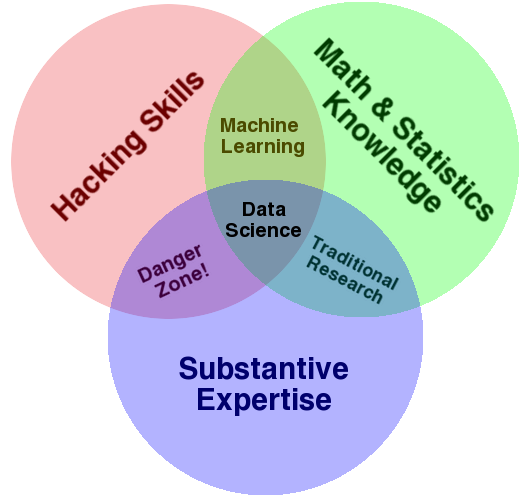
\includegraphics[width = 6cm]{./images/Data_Science_VD.png}
%%     \caption{\url{https://s3.amazonaws.com/aws.drewconway.com/viz/venn_diagram/data_science.html}}
%%   \end{figure}
%% \end{frame}

%% \note{
%%   Pragmatischere Sicht: \\
%%   Machine Learning ist die Schnittstelle zwischen Computer Science und Statistik.
%% }

\begin{frame}[plain]
  \addtocounter{framenumber}{-1}
  D.R. Cox in der Antwort auf Breiman's Paper: \\
  \vspace{0.5cm}
  \doublequoted{
    Descriptively appealing and transparent methods with a firm model base are the ideal.
  }
\end{frame}


\begin{frame}[plain]
  \addtocounter{framenumber}{-1}
  B. Efron in der Antwort auf Breiman's Paper: \\
\vspace{0.5cm}
  \doublequoted{
    we are being asked to face problems that never heard of good experimental design
  } \\
  Allerdings hält aber den Wert der Vorhersagegüte für überbewertet von Breiman. 

\end{frame}
\end{document}


